\section{Техническое задание}
\subsection{Основание для разработки}

Основанием для разработки является задание на выпускную квалификационную работу бакалавра Бизнес-проект «Внедрение цифровых технологий в сфере туризма. Разработка веб-приложения с картой туристических объектов региона».

\subsection{Цель и назначение разработки}

Разрабатываемое веб-приложение предназначено для предоставления пользователям — как жителям Курской области, так и приезжим туристам — интерактивной карты с отображением достопримечательностей, маршрутов и сервисов региона. Система будет выполнять роль цифрового гида, объединяя в себе навигационные, информационные и рекомендательные функции.

Целью разработки является создание удобного и адаптивного инструмента, позволяющего решать следующие задачи:
\begin{itemize}
	\item находить интересные туристические объекты по категории или местоположению;
	\item просматривать подробную информацию об объектах (описание, фотографии, режим работы, координаты);
	\item формировать персонализированные маршруты путешествий;
	\item сохранять избранные места и делиться маршрутами;
	\item использовать геолокацию для построения маршрутов от текущего местоположения;
	\item получать подсказки и уведомления в реальном времени (например, о времени работы или погодных условиях).
\end{itemize}

Актуальность проекта обусловлена следующими факторами:
\begin{itemize}
	\item стремительным ростом индивидуального туризма и интереса к самостоятельному планированию поездок;
	\item недостаточным уровнем цифровой представленности Курской области в туристической среде;
	\item потребностью в централизованной платформе, объединяющей разрозненные данные об объектах региона;
	\item трендом на развитие умного туризма (smart tourism), включающего использование картографических, информационных и рекомендательных систем.
\end{itemize}
Таким образом, проект направлен на решение комплексной задачи: повышение доступности туристической информации о Курской области средствами веб-технологий и улучшение пользовательского опыта при планировании и совершении путешествий.

\subsection{Требования к программной системе}
\subsubsection{Требования к данным программной системы}

Разрабатываемое веб-приложение предполагает активное взаимодействие с пользователем — как при просмотре и фильтрации туристических объектов, так и при построении маршрутов. В связи с этим необходимо определить формат\cite{b4}, источники и способы обработки как входной, так и выходной информации.

\begin{figure}[ht]
	\center{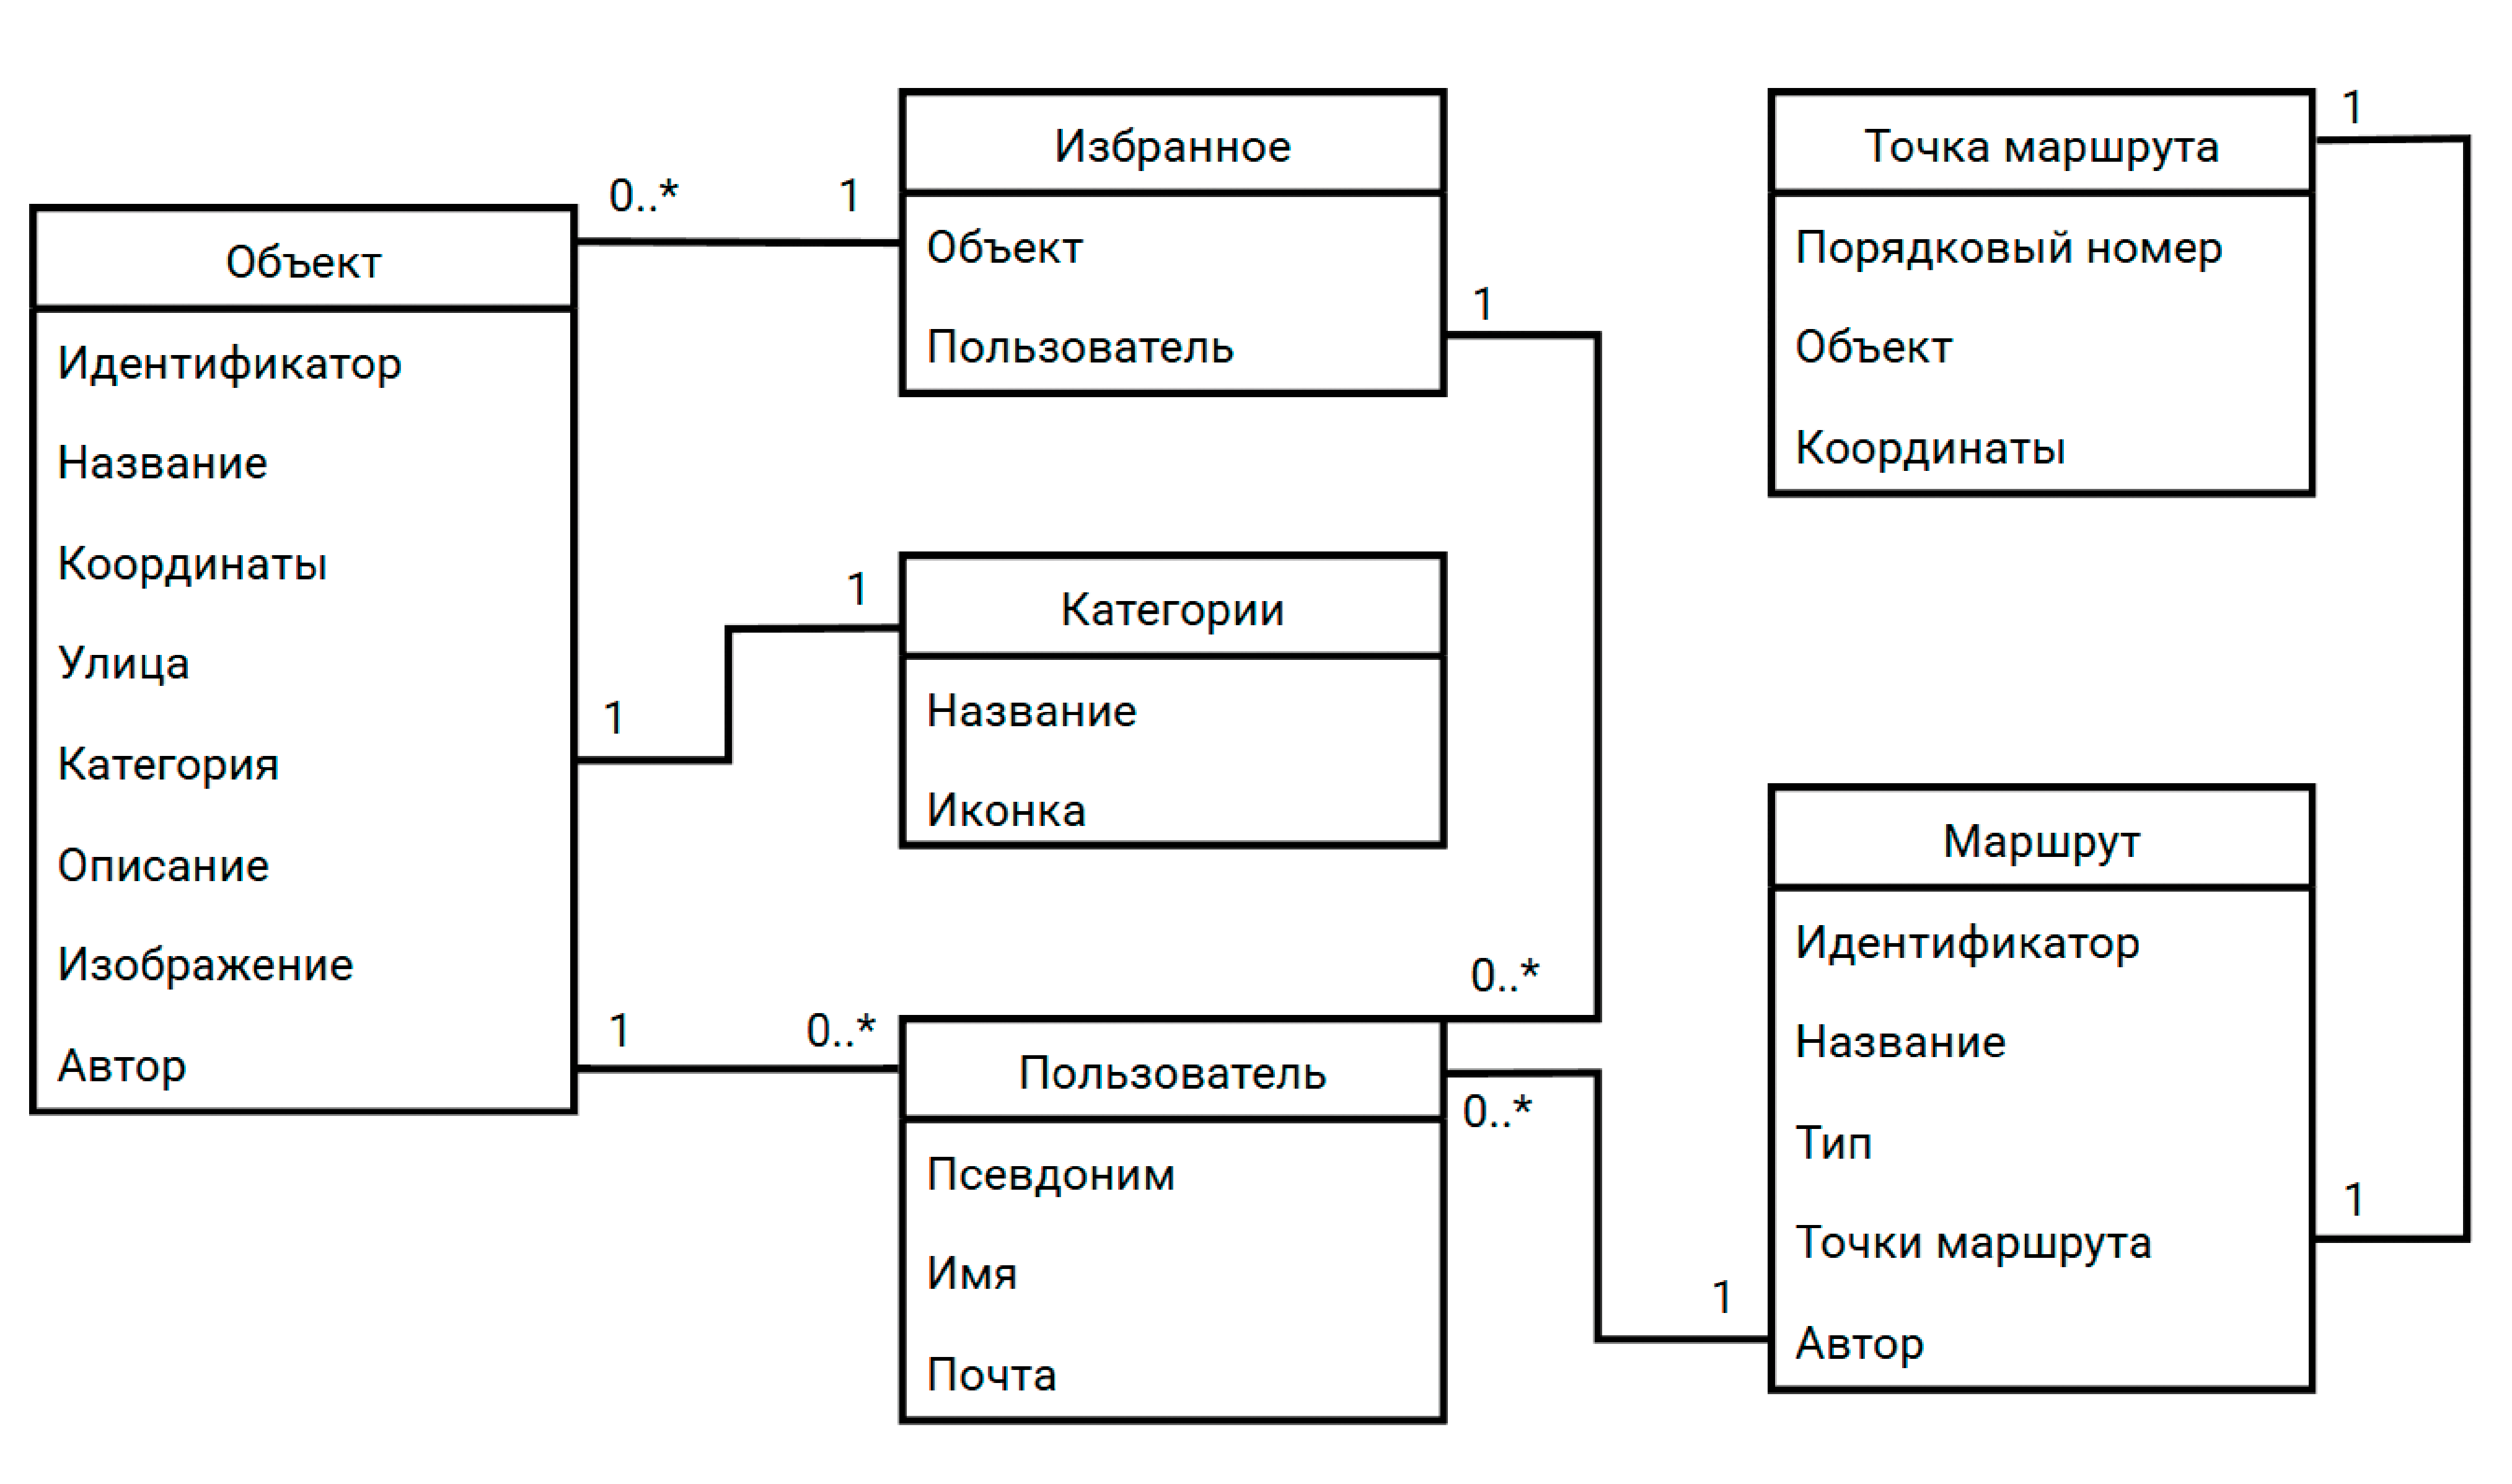
\includegraphics[width=1\linewidth]{comp}}
	\caption{Концептуальная модель данных}
	\label{comp:image}
\end{figure}

Вводимая информация:

Фильтрация объектов:
\begin{itemize}
	\item категория объекта (музеи, памятники, природные, религиозные и т. д.);
	\item уровень доступности (например, объекты с удобной парковкой, для людей с ОВЗ);
	\item расстояние от текущего местоположения.
\end{itemize}

Маршруты:
\begin{itemize}
	\item точка начала маршрута (может быть выбрана вручную или определена автоматически по геолокации);
	\item конечная и промежуточные точки (выбор из списка объектов или с карты);
	\item тип маршрута (пеший, автомобильный).
\end{itemize}

От внешних источников:
\begin{itemize}
	\item геолокация пользователя (через HTML5 API)\cite{b5};
	\item данные о достопримечательностях — из локальной базы или стороннего API;
	\item ответы от картографического сервиса (маршрутные данные).
\end{itemize}

Выводимая информация:

На главной и карте:
\begin{itemize}
	\item список доступных туристических объектов с краткой информацией\cite{b6} (название, категория, краткое описание);
	\item отображение объектов на карте (кастомные маркеры с всплывающими балунами);
	\item выделение объектов по фильтрам и поисковым запросам;
	\item визуальное отображение маршрута на карте с указанием начала, конца и промежуточных точек;
	\item подсказки/уведомления о текущем состоянии маршрута или выборе точек.
\end{itemize}

В балуне объекта:
\begin{itemize}
	\item название объекта;
	\item фотография или иконка;
	\item краткое описание;
	\item кнопки.
\end{itemize}

В панели маршрута:
\begin{itemize}
	\item адреса и названия всех точек маршрута;
	\item общая длина маршрута и ориентировочное время в пути;
	\item возможность изменения порядка точек;
	\item кнопка "Оптимизировать маршрут".
\end{itemize}

\subsubsection{Функциональные требования к программной системе}

Разрабатываемое веб-приложение должно обладать определённым набором функциональных возможностей, ориентированных на конечного пользователя — туриста. Основная задача системы — обеспечить удобный доступ к информации о туристических объектах Курской области и упростить процесс построения индивидуальных маршрутов\cite{b7}.

Основной функционал приложения:
\begin{enumerate}
	\item Отображение туристических объектов на карте.
	\item Возможность фильтрации объектов по категориям.
	\item Просмотр информации о выбранном объекте.
	\item Формирование персонального маршрута.
	\item Добавление точек маршрута вручную из списка или карты.
	\item Поддержка промежуточных точек и автоматическая прокладка оптимального пути.
	\item Выбор типа маршрута (пеший, автомобильный и др.).
	\item Автоматическое определение начальной точки (геолокация пользователя).
	\item Возможность редактирования порядка следования точек (перетаскивание, удаление).
	\item Возможность добавления/удаления объектов или маршрутов в избранное.
	\item Просмотр списка избранных точек на отдельной вкладке.
	\item Получение текущего местоположения пользователя с разрешения.
	\item Визуальное сопровождение движения по маршруту.
\end{enumerate}

На рисунке ~\ref{templ:image} в виде диаграммы прецедентов представлены функции, доступные всем пользователям.

На рисунке ~\ref{templauto:image} представлены дополнительные функции для авторизованных пользователей.

\begin{figure}[ht]
	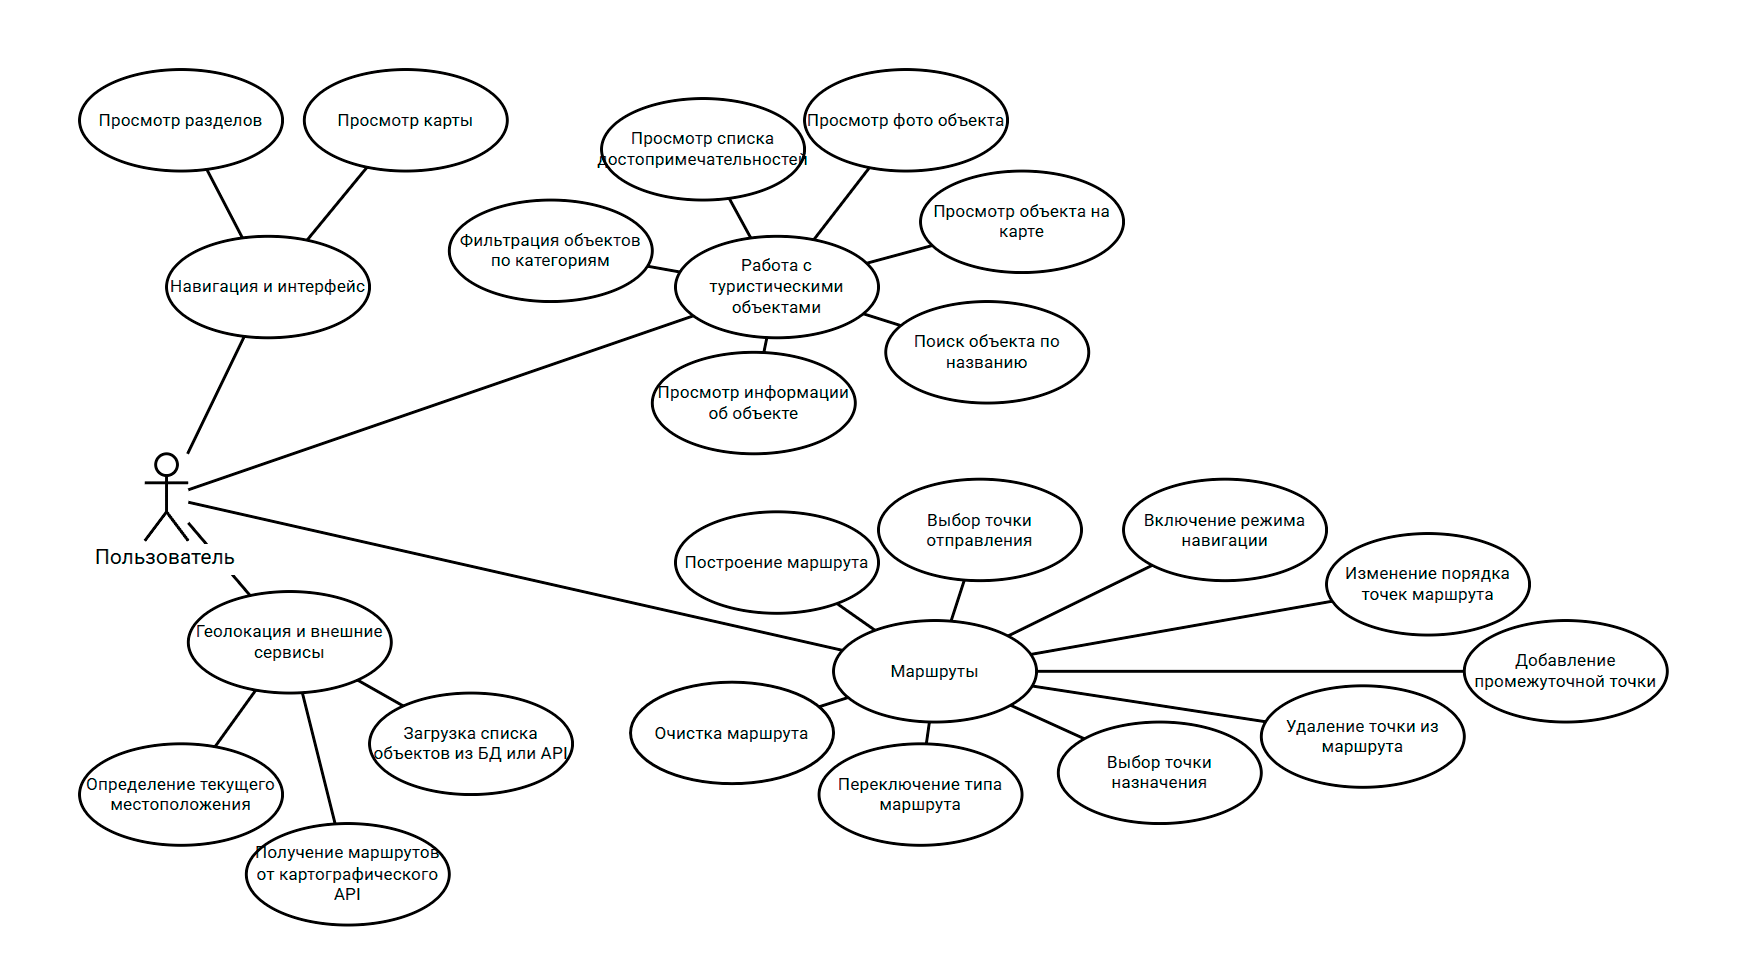
\includegraphics[width=1\linewidth]{templ}
	\caption{Диаграмма прецедентов}
	\label{templ:image}
\end{figure}

\vspace{+100mm}
\begin{figure}[ht]
	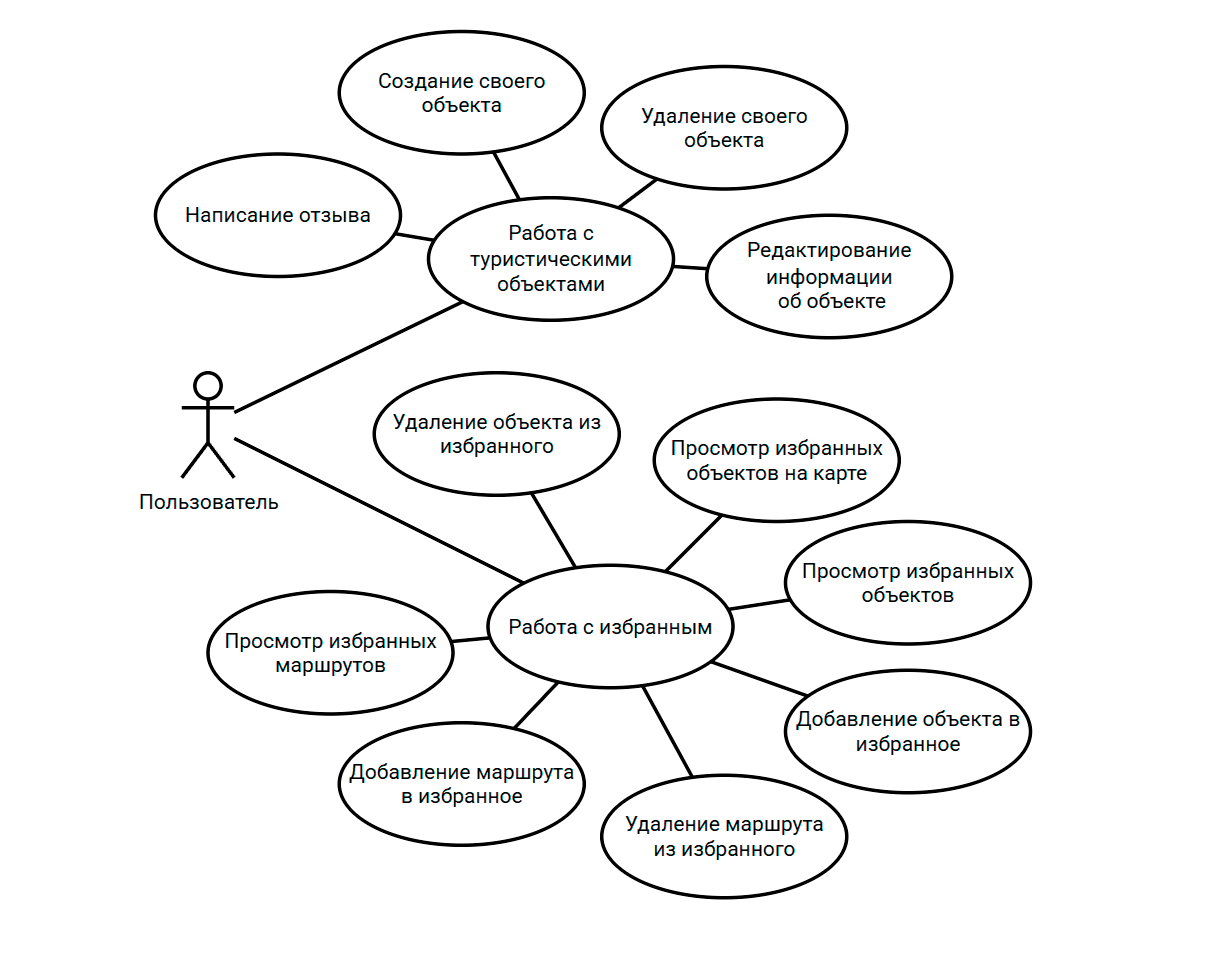
\includegraphics[width=1\linewidth]{templauto}
	\caption{Диаграмма прецедентов для авторизованного пользователя}
	\label{templauto:image}
\end{figure}

\subsubsection{Моделирование вариантов использования}
\paragraph{Вариант использования «Построение маршрута между туристическими объектами»}

Основной исполнитель: Пользователь

Заинтересованные лица и их требования:

Пользователь: хочет быстро построить удобный маршрут между выбранными достопримечательностями.

Система: должна обработать маршрут с учётом географических координат.

Предусловие: Пользователь выбрал как минимум две точки на карте.

Постусловие: Маршрут успешно построен и отображён на карте.

Основной успешный сценарий:
\begin{enumerate}
	\item Пользователь выбирает начальную и конечную точки.
	\item При необходимости добавляет промежуточные точки.
	\item Устанавливает тип маршрута (пеший или автомобильный).
	\item Система запрашивает маршрут у внешнего API.
	\item Построенный маршрут отображается на карте с указанием всех точек.
\end{enumerate}

\paragraph{Вариант использования «Фильтрация туристических объектов по категории»}

Основной исполнитель: Пользователь

Заинтересованные лица и их требования:

Пользователь: хочет отобразить только определённый тип объектов (например, музеи).

Система: обязана быстро применить фильтр и обновить карту.

Предусловие: Пользователь находится на странице карты.

Постусловие: На карте и в списке отображаются только объекты выбранной категории.

Основной успешный сценарий:
\begin{enumerate}
	\item Пользователь открывает панель фильтров.
	\item Отмечает нужные категории (одну или несколько).
	\item Система скрывает неактуальные объекты и обновляет видимость.
	\item Пользователь видит только интересующие его объекты.
\end{enumerate}

\paragraph{Вариант использования «Добавление объекта в избранное»}

Основной исполнитель: Авторизованный пользователь

Заинтересованные лица и их требования:

Пользователь: хочет сохранить интересные места для повторного просмотра.

Система: обязана привязать объект к конкретному пользователю.

Предусловие: Пользователь авторизован и открыл карточку объекта.

Постусловие: Объект сохранён в избранном пользователя.

Основной успешный сценарий:
\begin{enumerate}
	\item Пользователь открывает балун объекта.
	\item Нажимает кнопку "Добавить в избранное".
	\item Система отправляет данные на сервер.
	\item Сервер сохраняет связь между пользователем и объектом.
	\item Пользователь получает подтверждение об успешном добавлении.
\end{enumerate}

\paragraph{Вариант использования «Поиск объекта по ключевому слову»}

Основной исполнитель: Пользователь

Заинтересованные лица и их требования:

Пользователь: хочет быстро найти конкретную достопримечательность по названию.

Система: обязана предоставить релевантные результаты.

Предусловие: Пользователь находится на карте или в списке объектов.

Постусловие: Пользователь видит подходящие объекты на карте и/или в списке.

Основной успешный сценарий:
\begin{enumerate}
	\item Пользователь вводит ключевое слово в поисковую строку.
	\item Система фильтрует объекты, соответствующие запросу.
	\item Отображаются подходящие результаты.
	\item Пользователь может кликнуть по объекту для получения информации.
\end{enumerate}

\paragraph{Вариант использования «Определение текущего местоположения пользователя»}

Основной исполнитель: Пользователь

Заинтересованные лица и их требования:

Пользователь: хочет увидеть своё текущее местоположение на карте.

Система: обязана корректно запросить и отобразить координаты.

Предусловие: Пользователь дал разрешение на доступ к геолокации.

Постусловие: На карте отображается текущее местоположение пользователя.

Основной успешный сценарий:
\begin{enumerate}
	\item Пользователь нажимает кнопку "Отображать местоположение".
	\item Браузер запрашивает разрешение на доступ к геолокации.
	\item Пользователь разрешает.
	\item Система получает координаты и отображает метку на карте.
	\item Центр карты сдвигается на позицию пользователя.
\end{enumerate}

\paragraph{Вариант использования «Сохранение маршрута в личный кабинет»}

Основной исполнитель: Авторизованный пользователь

Заинтересованные лица и их требования:

Пользователь: хочет сохранить построенный маршрут для дальнейшего использования.

Система: должна обеспечить хранение маршрутов с возможностью последующего редактирования.

Предусловие: Пользователь авторизован и построил маршрут.

Постусловие: Маршрут сохранён в базе данных и доступен в профиле пользователя.

Основной успешный сценарий:
\begin{enumerate}
	\item Пользователь строит маршрут.
	\item Нажимает кнопку "Сохранить маршрут".
	\item Вводит название маршрута.
	\item Система отправляет маршрут на сервер.
	\item Сервер сохраняет маршрут, возвращает подтверждение.
	\item Пользователь видит сохранённый маршрут в личном кабинете.
\end{enumerate}

\paragraph{Вариант использования «Просмотр информации о достопримечательности»}

Основной исполнитель: Пользователь

Заинтересованные лица и их требования:

Пользователь: хочет узнать подробную информацию о конкретной точке интереса.

Администратор контента: ожидает, что пользователи получают корректные и актуальные сведения.

Предусловие: Пользователь нажал на объект на карте.

Постусловие: Открыта подробная карточка объекта с текстом, фото и ссылками.

Основной успешный сценарий:
\begin{enumerate}
	\item Пользователь кликает по маркеру на карте.
	\item Система отображает всплывающее окно (балун).
	\item Пользователь переходит к подробной карточке объекта.
	\item В карточке отображаются: название, описание, фото, категория, адрес, часы работы и др.
\end{enumerate}

\paragraph{Вариант использования «Сброс маршрута»}

Основной исполнитель: Пользователь

Заинтересованные лица и их требования:

Пользователь: хочет очистить текущие настройки, чтобы начать с чистого листа.

Система: должна корректно сбросить все активные параметры без сбоев.

Предусловие: Активен фильтр категорий или построен маршрут.

Постусловие: На карте отображаются все объекты, маршрут удалён.

Основной успешный сценарий:
\begin{enumerate}
	\item Пользователь закрывает панель настройки маршрута.
	\item Система удаляет маршрут с карты.
	\item Отображаются все объекты по умолчанию.
	\item Пользователь может начать новый поиск.
\end{enumerate}

\paragraph{Вариант использования «Перемещение точек маршрута вручную»}

Основной исполнитель: Пользователь

Заинтересованные лица и их требования:

Пользователь: хочет настроить порядок прохождения точек.

Система: должна позволить интерактивное изменение порядка точек.

Предусловие: Построен маршрут с несколькими точками.

Постусловие: Новый порядок точек сохранён, маршрут перестроен.

Основной успешный сценарий:
\begin{enumerate}
	\item Пользователь переходит к редактированию маршрута.
	\item Перетаскивает точки в нужном порядке.
	\item Система перестраивает маршрут.
	\item Новый маршрут отображается на карте.
\end{enumerate}

\paragraph{Вариант использования «Просмотр избранных объектов на карте»}

Основной исполнитель: Авторизованный пользователь

Заинтересованные лица и их требования:

Пользователь: хочет быстро отобразить все сохранённые объекты на карте.

Система: должна отобразить только объекты, находящиеся в избранном.

Предусловие: У пользователя есть добавленные в избранное объекты.

Постусловие: На карте отображаются маркеры только для избранных точек.

Основной успешный сценарий:
\begin{enumerate}
	\item Пользователь открывает раздел "Избранное".
	\item Нажимает кнопку "Показать на карте".
	\item Система запрашивает список избранных объектов.
	\item На карте появляются только эти точки.
	\item Карта центрируется на области с избранными.
\end{enumerate}

\paragraph{Вариант использования «Выбор типа маршрута»}

Основной исполнитель: Пользователь

Заинтересованные лица и их требования:

Пользователь: хочет выбрать наиболее удобный способ передвижения.

Система: должна перестроить маршрут с учётом выбранного типа.

Предусловие: Построен маршрут или выбраны точки.

Постусловие: На карте отображается актуальный маршрут соответствующего типа.

Основной успешный сценарий:
\begin{enumerate}
	\item Пользователь строит маршрут или выбирает точки.
	\item В интерфейсе выбирает тип маршрута (пеший или автомобильный).
	\item Система отправляет запрос в API с параметром типа маршрута.
	\item Полученный маршрут обновляется на карте.
	\item Пользователь получает маршрут, подходящий под выбранный режим.
\end{enumerate}

\paragraph{Вариант использования «Авторизация пользователя»}

Основной исполнитель: Пользователь

Заинтересованные лица и их требования:

Пользователь: хочет получить доступ к персональным функциям — избранному, сохранённым маршрутам.

Система: должна обеспечить безопасный вход и защиту данных.

Предусловие: Пользователь находится на сайте и не авторизован.

Постусловие: Пользователь авторизован и получает доступ к личным данным.

Основной успешный сценарий:
\begin{enumerate}
	\item Пользователь открывает форму авторизации.
	\item Вводит логин и пароль.
	\item Система проверяет данные и выдаёт токен.
	\item Открывается интерфейс с доступом к личному кабинету.
	\item Пользователь может работать с избранным и маршрутами.
\end{enumerate}

\paragraph{Вариант использования «Получение пошаговых инструкций к маршруту»}

Основной исполнитель: Пользователь

Заинтересованные лица и их требования:

Пользователь: хочет получить подробные указания по движению.

Система: должна предоставить навигационные шаги, основанные на маршруте.

Предусловие: Построен маршрут.

Постусловие: Пользователь видит текстовые инструкции по маршруту.

Основной успешный сценарий:
\begin{enumerate}
	\item Пользователь строит маршрут.
	\item Нажимает кнопку "Показать подробности".
	\item Система запрашивает информацию у картографического API.
	\item Отображается список шагов (поворотов, расстояний, ориентиров).
	\item Пользователь может следовать инструкции во время путешествия.
\end{enumerate}

\paragraph{Вариант использования «Просмотр подробной статистики о маршруте»}

Основной исполнитель: Пользователь

Заинтересованные лица и их требования:

Пользователь: хочет оценить длину, продолжительность, количество объектов на маршруте.

Система: должна проанализировать маршрут и отобразить метрики.

Предусловие: Маршрут построен.

Постусловие: Отображается статистика маршрута.

Основной успешный сценарий:
\begin{enumerate}
	\item Пользователь строит маршрут.
	\item Открывает вкладку с информацией.
	\item Система вычисляет: общее расстояние, количество точек, примерное время в пути.
	\item Отображает результаты в удобном формате.
	\item Пользователь принимает решение о корректировке или сохранении маршрута.
\end{enumerate}

\paragraph{Вариант использования «Оставление отзыва о туристическом объекте»}

Основной исполнитель: Авторизованный пользователь

Заинтересованные лица и их требования:

Пользователь: хочет поделиться впечатлениями о достопримечательности.

Администратор: стремится собирать обратную связь и отображать рейтинги.

Предусловие: Пользователь авторизован и посетил страницу объекта.

Постусловие: Отзыв сохранён и отображается в карточке объекта.

Основной успешный сценарий:
\begin{enumerate}
	\item Пользователь переходит на страницу объекта.
	\item Нажимает "Оставить отзыв".
	\item Заполняет форму с текстом и рейтингом.
	\item Система сохраняет отзыв в базу данных.
	\item Отзыв отображается другим пользователям.
\end{enumerate}

\paragraph{Вариант использования «Загрузка пользовательского объекта на карту»}

Основной исполнитель: Авторизованный пользователь

Заинтересованные лица и их требования:

Пользователь: хочет добавить малоизвестное или новое туристическое место.

Администратор: требует предварительной модерации перед публикацией.

Предусловие: Пользователь авторизован.

Постусловие: Объект добавлен в систему и ожидает модерации.

Основной успешный сценарий:
\begin{enumerate}
	\item Пользователь нажимает "Добавить объект".
	\item Заполняет форму с координатами, описанием, фото.
	\item Отправляет заявку.
	\item Система сохраняет данные и уведомляет модератора.
	\item После одобрения объект становится видимым другим пользователям.
\end{enumerate}

\paragraph{Вариант использования «Получение рекомендаций по маршрутам»}

Основной исполнитель: Пользователь

Заинтересованные лица и их требования:

Пользователь: хочет быстро получить готовые маршруты по своим интересам.

Система: должна учитывать предпочтения и текущие условия (время, погоду).

Предусловие: Пользователь указал интересы и параметры маршрута.

Постусловие: Отображаются подходящие готовые маршруты.

Основной успешный сценарий:
\begin{enumerate}
	\item Пользователь открывает раздел "Рекомендации".
	\item Выбирает интересующие категории и желаемую длительность.
	\item Система анализирует возможные маршруты.
	\item Показывает список наиболее подходящих.
	\item Пользователь выбирает и открывает один из маршрутов на карте.
\end{enumerate}

\paragraph{Вариант использования «Построение кольцевого маршрута»}

Основной исполнитель: Пользователь

Заинтересованные лица и их требования:

Пользователь: хочет маршрут, начинающийся и заканчивающийся в одной точке.

Система: должна правильно обработать алгоритм кольцевого построения.

Предусловие: Задана стартовая точка и фильтр интересов.

Постусловие: Отображается кольцевой маршрут на карте.

Основной успешный сценарий:
\begin{enumerate}
	\item Пользователь выбирает "Кольцевой маршрут".
	\item Вводит начальную точку и интересующие категории.
	\item Указывает допустимую длину/время маршрута.
	\item Система формирует кольцевой маршрут по заданным параметрам.
	\item Пользователь получает визуализацию маршрута и может начать навигацию.
\end{enumerate}

\paragraph{Вариант использования «Удаление точки маршрута»}

Основной исполнитель: Пользователь

Заинтересованные лица и их требования:

Пользователь: хочет исключить ненужную точку из маршрута.

Система: должна корректно пересчитать маршрут.

Предусловие: У пользователя открыт маршрут с несколькими точками.

Постусловие: Точка удалена, маршрут перестроен.

Основной успешный сценарий:
\begin{enumerate}
	\item Пользователь открывает список точек маршрута.
	\item Нажимает иконку удаления рядом с нужной точкой.
	\item Система удаляет точку из списка.
	\item Выполняется пересчёт маршрута.
	\item Новый маршрут отображается на карте. навигацию.
\end{enumerate}

\paragraph{Вариант использования «Оптимизация порядка точек маршрута по времени и расстоянию»}

Основной исполнитель: Пользователь

Заинтересованные лица и их требования:

Пользователь: хочет сэкономить время в пути, оптимизируя маршрут.

Система: должна автоматически пересчитать маршрут с наименьшими затратами по времени/расстоянию.

Предусловие: У пользователя уже создан маршрут с несколькими точками.

Постусловие: Система перестроила маршрут, изменив порядок точек для оптимального прохождения.

Основной успешный сценарий:
\begin{enumerate}
	\item Пользователь открывает сохранённый или текущий маршрут.
	\item Нажимает кнопку «Оптимизировать маршрут».
	\item Система анализирует возможные перестановки точек.
	\item Выполняется выбор наилучшего варианта с учётом расстояния и/или времени.
	\item Отображается обновлённый маршрут, пользователь может его сохранить или начать навигацию.
\end{enumerate}

\subsubsection{Требования к пользовательскому интерфейсу}

Интерфейс разрабатываемого веб-приложения должен быть визуально лёгким и адаптированным под широкую аудиторию\cite{b8} — от молодёжи до пожилых людей, путешествующих по Курской области. Основное внимание уделяется удобству взаимодействия, минимизации числа действий для выполнения ключевых операций, а также визуальной согласованности всех элементов.

Основными компонентами\cite{b9} интерфейса являются:
\begin{enumerate}
	\item Интерактивная карта региона, на которой отображаются туристические объекты. Карта  занимает центральное место в интерфейсе, так как с ней связано основное взаимодействие пользователя — поиск интересных мест, добавление точек маршрута и просмотр информации о достопримечательностях. Все элементы управления, связанные с картой, должны располагаться так, чтобы не перекрывать её значимую часть, при этом оставаться легко доступными.
	\item Панель фильтрации объектов. Она позволяет пользователю выбирать категории достопримечательностей, такие как музеи, архитектурные памятники, природные объекты и т. д.
	\item Форма построения маршрута. Она представляет собой всплывающее окно с полями «откуда», «куда» и возможностью добавления промежуточных точек.
	\item Карточка объекта. Она открывается при клике по метке на карте и в ней отображаются основная информация (название, фотография, описание), а также кнопки действий: добавление в маршрут, добавление в избранное, получение подробностей.
	\item Личный кабинет. В нем пользователь может просматривать сохранённые маршруты и избранные объекты.
\end{enumerate}

Интерфейс реализован на русском языке. Так же присутствует возможность реализации английской версии (в перспективе).

\subsubsection{Нефункциональный требования к программной системе}
\paragraph{Требования к надёжности}

Для обеспечения корректной и безопасной работы веб-приложения необходимо предусмотреть комплекс технических и организационных мер\cite{b10}, направленных на защиту пользовательских данных, устойчивость системы к ошибкам, сбоям и потенциальным угрозам со стороны злоумышленников.

Надёжность предполагает стабильную работу приложения в условиях стандартной пользовательской нагрузки, а также корректное поведение при возникновении нештатных ситуаций.

В рамках данного проекта под надёжностью понимается следующее:
\begin{enumerate}
	\item Обработка ошибок.	Все потенциальные ошибки (например, недоступность карты, сбои подключения к API, ошибки загрузки данных) должны обрабатываться с выводом понятного уведомления для пользователя без прекращения работы интерфейса.
	\item Валидация данных.	Все вводимые или получаемые извне данные должны проходить многоуровневую проверку на клиентской и серверной сторонах, что исключает возможность ошибок в логике или отображении.
	\item Резервирование критических элементов.	При использовании внешних API (например, картографических) рекомендуется реализовать fallback-механизмы или локальное кеширование часто используемых данных.
	\item Логирование. Серверная часть должна вести журнал событий (ошибок, действий пользователя, обращений к API) с целью оперативной диагностики и предотвращения сбоев.
\end{enumerate}

\paragraph{Требования к безопасности}

Безопасность данных пользователей, включая маршруты, избранное и потенциальную информацию о местоположении, является ключевым требованием. Для защиты информации применяются следующие меры:
\begin{enumerate}
	\item Шифрование трафика. Вся передача данных между клиентом и сервером должна осуществляться по протоколу HTTPS с использованием SSL/TLS-сертификатов.
	\item Контроль доступа. Регистрация и вход должны выполняться с защитой от подбора паролей (ограничение попыток, капча). Должны осуществляться хеширование паролей в базе данных (с применением алгоритмов bcrypt или Argon2) и защита пользовательских маршрутов и данных от несанкционированного доступа (привязка к сессии или токену).
	\item Защита от распространённых атак. 
	
	XSS (межсайтовый скриптинг): фильтрация HTML-содержимого в пользовательском вводе.
	
	CSRF (межсайтовая подделка запроса): защита форм с помощью токенов.
	
	SQL-инъекции: использование подготовленных запросов и ORM.
	
	CORS: настройка политик кросс-доменных запросов с ограничением доверенных источников.
\end{enumerate}

\paragraph{Требования к программной и аппаратной среде}

Для корректной работы и стабильного функционирования веб-приложения по отображению туристических объектов Курской области с функцией маршрутизации требуется соблюдение определённых условий по программной и аппаратной среде. Ниже приведены минимальные и рекомендуемые параметры для клиентской и серверной сторон.

Программные требования:

Клиентская часть (устройство пользователя):
\begin{itemize}
	\item операционные системы: Windows 10+, macOS 11+, Android 8.0+, iOS 13+;
	\item браузеры (актуальные версии): Google Chrome, Mozilla Firefox, Safari, Microsoft Edge;
	\item поддержка JavaScript и включённые cookie обязательны.
\end{itemize}

Серверная часть (хостинг или VPS):
\begin{itemize}
	\item операционная система: Ubuntu Server 20.04+ / Debian 11+ / CentOS 8+;
	\item веб-сервер: Apache (с поддержкой HTTPS);
	\item язык серверной логики: PHP (v8+);
	\item база данных: MySQL 8.0+;
	\item API и внешние сервисы: Яндекс.Карты API\cite{b11}.
\end{itemize}

Аппаратные требования:

Клиентское устройство:
\begin{itemize}
	\item процессор: двухъядерный от 1.5 ГГц;
	\item оперативная память: от 2 ГБ;
	\item разрешение экрана: от 1280×720.
\end{itemize}

Сервер:

Минимальные характеристики для пилотной версии:
\begin{itemize}
	\item CPU: 2 vCPU;
	\item RAM: 2–4 ГБ;
	\item SSD: от 20 ГБ;
	\item канал: не менее 100 Мбит/с.
\end{itemize}

Рекомендуемые характеристики для масштабируемой версии:
\begin{itemize}
	\item CPU: 4 vCPU и выше;
	\item RAM: 8 ГБ и выше;
	\item SSD: 40+ ГБ с возможностью масштабирования;
	\item резервное копирование данных раз в сутки.
\end{itemize}

\subsection{Требования к оформлению документации}

Разработка программной документации и программного изделия должна производиться согласно ГОСТ 19.102-77 и ГОСТ 34.601-90. Единая система программной документации.

Программная документация включает в себя:
\begin{enumerate}
	\item Анализ предметной области.
	\item Техническое задание.
	\item Технический проект.
	\item Рабочий проект.
\end{enumerate}
